\chapter{Many-body physical systems}

\todo{For now only some notations are written down}

\section{Classical systems}

In this thesis, we mainly focus on systems consisting of spin-$\frac{1}{2}$ particles, and most results are generalizable to higher spins, fermions, and bosons.

To study a classical system of $N$ spins, we first characterize its microscopic properties using the Hamiltonian function $H(\vs)$, which defines the microscopic energy given the system configuration $\vs$. Here $\vs$ is a vector of $N$ entries $(s_1, s_2, \ldots, s_N)$, and each entry $s_i$ can be either $+1$ or $-1$, representing spin up and down respectively.

Then we consider an ensemble of many possible configurations of the system following the distribution $p(\vs)$. When the system is at the temperature $T$ in thermal equilibrium, $p(\vs)$ is given by the Boltzmann distribution
\begin{equation}
p_\text{B}(\vs) = \frac{\rme^{-\beta H(\vs)}}{Z},
\label{eq:boltzmann}
\end{equation}
where $\beta = \frac{1}{T}$ is the inverse temperature, and
\begin{equation}
Z = \sum_\vs \rme^{-\beta H(\vs)}
\end{equation}
is the partition function that normalizes the distribution.

Knowing the distribution of the configurations, we can obtain the macroscopic expectation value of any physical observable $O$ by
\begin{equation}
\bar{O} = \sum_\vs p(\vs) O(\vs).
\label{eq:cl-obs}
\end{equation}

The observables of common interest include the energy $E$, the heat capacity $\calC_V$, the magnetization $M$, the magnetic susceptibility $\chi_M$, and the spin correlations $C_{i j}$.

Free energy $F = -T \ln Z = E - T S$

Entropy $S = -\sum_\vs p(\vs) \ln p(\vs)$

Ground state $\vs_0 = \arg\min_\vs H(\vs)$

Ground state energy $E_0 = \min_\vs H(\vs) = \lim_{T \to 0} E$

The analytical method to calculate the observable is known only in some cases of simple systems. Many 1D classical systems are solvable using the transfer matrix method~\cite{chaikin1995principles5}, with a few 2D classical and 1D quantum results such as the celebrated Onsager's solution for the 2D Ising model~\cite{onsager1944crystal, baxter1995solvable,march2016exactly, caravelli2022some}. In the remaining cases that constitute rich and unknown physical phenomena, numerical methods are required to compute them.

The summation in \cref{eq:cl-obs} runs over $2^N$ possible configurations of the system in total, which is exponentially large and quickly becomes intractable as $N$ increases. As of this writing, the largest supercomputers in the world have peak computational power in the order of $10^{18}$ floating point operations per second ($1$ exaFLOPS)~\cite{kogge2022frontier}, which can sum over only $81$ spins in the ``reasonable'' time budget of a month, even if the summation is unrealistically optimized to take one floating point operation for each configuration, and other costs such as the storage are ignored. Therefore, we can only resort to approximation methods to compute the expectation in practice, which we will discuss in the following chapters.

Computational complexity of computing $Z$, so smart exact methods are not much better than brute force

\subsection{Classical Ising model}

The Ising model with general interactions $J_{i j}$:
\begin{equation}
H(\vs) = \sum_{i, j} J_{i j} s_i s_j.
\label{eq:cl-ising-general}
\end{equation}
In this thesis, we omit the external fields for simplicity.

In the simplest case, we only consider uniform nearest neighbor interactions, and omit the external fields:
\begin{equation}
H(\vs) = J \sum_{\langle i, j \rangle} s_i s_j,
\label{eq:cl-ising}
\end{equation}
where $\langle i, j \rangle$ runs over nearest neighbors, and we assume $J = 1$ unless stated otherwise.

We can also consider local interactions beyond nearest neighbors, which depend on the distance:
\begin{equation}
H(\vs) = J_1 \sum_{\langle i, j \rangle} s_i s_j + J_2\!\sum_{\llangle i, j \rrangle}\!s_i s_j + J_3\!\!\sum_{\langle\!\langle\!\langle i, j \rangle\!\rangle\!\rangle}\!\!s_i s_j \ldots
\label{eq:cl-ising-nnn}
\end{equation}

Square lattice and triangular lattice, geometrical frustration

Open boundary conditions (OBC) and periodic boundary conditions (PBC)

Disorder in $J$

\subsection{Hopfield model}

The Hopfield model~\cite{hopfield1982neural, amit1985spin} is a model of associative memory. It is defined by the Ising model in \cref{eq:cl-ising-general} with the interactions
\begin{equation}
J_{i j} = -\frac{1}{N} \sum_{p = 1}^{n_\text{p}} \xi^{(p)}_i \xi^{(p)}_j,
\label{eq:hopfield}
\end{equation}
where $\{\vxi^{(1)}, \vxi^{(2)}, \ldots, \vxi^{(n_\text{p})}\}$ are some special spin configurations, known as the ``patterns'', and $n_\text{p}$ is the number of patterns. We define the overlap between two configurations:
\begin{equation}
\ip{\vs}{\vs'} = \frac{1}{N} \sum_i s_i s'_i.
\label{eq:cl-overlap}
\end{equation}
The patterns need to be orthogonal:
\begin{equation}
\ip{\vxi^{(p)}}{\vxi^{(q)}} = 0, \quad \forall p, q.
\end{equation}
The model has $2 n_\text{p}$ degenerate ground states: $\vs_0 = \pm \vxi^{(p)}$, $H(\vs_0) = -N$. Therefore, we say the model ``memorizes'' the patterns.

\subsection{Sherrington--Kirkpatrick (SK) model}
\label{sec:sk}

The Sherrington--Kirkpatrick (SK) model is defined by the Ising model in \cref{eq:cl-ising-general} with each interaction $J_{i j}$ sampled from a Gaussian distribution with zero mean and a variance of $\frac{1}{N}$.

\subsection{Frustrated plaquette model}

The 2D frustrated plaquette model (FPM)
\begin{align}
H(\vs) = &\phantom{{}+{}} J_1 \sum_{i, j = 1}^L s_{i, j} (s_{i + 1, j} + s_{i, j + 1}) \nonumber \\
&+ J_3 \sum_{i, j = 1}^L s_{i, j} (s_{i + 2, j} + s_{i, j + 2}) \nonumber \\
&+ K \sum_{i, j = 1}^L s_{i, j} \, s_{i + 1, j} \, s_{i, j + 1} \, s_{i + 1, j + 1},
\label{eq:fpm}
\end{align}

\begin{figure}[htb]
\centering
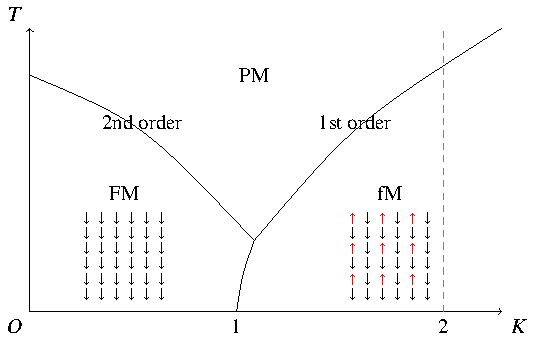
\includegraphics[width=0.7\linewidth]{ch2/fpm_phase.pdf}
\caption[Phase diagram for frustrated plaquette model]{
Sketch of the phase diagram for the frustrated plaquette model (FPM) with $J_1 = J_3 = -1$.
Examples of the ground state in the ferromagnetic (FM) and the ferrimagnetic (fM) phases are shown respectively.
The first-order phase transition at $K = 2$ is studied in Ref.~\cite{wu2021unbiased}, as indicated by the dashed vertical line.
This figure is reproduced from Fig.~3~(a) in Ref.~\cite{wu2021unbiased}.
}
\label{fig:fpm-phase}
\end{figure}

\section{Quantum systems}

In the quantum case, we start from studying the ground state, or zero temperature properties of a system. The quantum state $\ket{\psi}$ of the system can be represented in the computational basis by
\begin{equation}
\ket{\psi} = \sum_\vs \psi(\vs) \ket{\vs},
\end{equation}
where $\vs$ is a vector of $N$ classical spin values, which is a possible outcome if we measure the quantum system along a chosen $z$ direction. The basis states $\{\ket{\vs}\}$ satisfy the orthonormal relation $\ip{\vs}{\vs'} = \delta_{\vs, \vs'}$, so we can project the state $\ket{\psi}$ onto a basis state $\ket{\vs}$ and obtain the corresponding wave function value $\psi(\vs) = \ip{\vs}{\psi}$, which is a complex number in general. Therefore, the state $\ket{\psi}$ is a complex vector in the Hilbert space of $2^N$ dimensions. Moreover, it needs to satisfy the normalization condition $\ip{\psi}{\psi} = \sum_{\vs} |\psi(\vs)|^2 = 1$.

When the system is at the ground state, it is characterized by the Hamiltonian operator $\hat{H}$:
\begin{equation}
\ket{\psi_0} = \arg\min_{\ket{\psi}} \mel{\psi}{\hat{H}}{\psi}.
\label{eq:gs}
\end{equation}
In contrast to the classical case, even if the quantum system is at the ground state and is non-degenerate, it can still be a superposition of exponentially many basis states.

Knowing the quantum state of the system, we can obtain the expectation value of any physical observable $\hat{O}$ by
\begin{equation}
\bar{O} = \mel{\psi}{\hat{O}}{\psi} = \sum_{\vs, \vs'} \psi^*(\vs) O(\vs, \vs') \psi(\vs),
\label{eq:qu-obs}
\end{equation}
where $O(\vs, \vs') = \mel{\vs}{\hat{O}}{\vs'}$. Like the classical case, the summation in \cref{eq:qu-obs} also contains exponentially many terms and is intractable. Worse still, to exactly compute the ground state vector in \cref{eq:gs} in general, one needs the exact diagonalization (ED) of the $2^N \times 2^N$ Hamiltonian matrix, which takes even higher exponential time~\cite{weisse2008exact}. Therefore, we again need approximation methods to study the system in practice.

Beyond the ground state, the quantum system can be a mixed state characterized by a density matrix, and represented in the eigenbasis by
\begin{equation}
\hat{\rho} = \sum_i p_i \ket{\psi_i}\bra{\psi_i},
\end{equation}
where $\ket{\psi_i}$ is the $i$-th lowest eigenstate of the Hamiltonian, and $p_i$ is the corresponding probability of measuring this state. When the system is at the temperature $T$ in thermal equilibrium, $p_i$ is given by the Boltzmann distribution. Knowing the density matrix, we can obtain the expectation value of any physical observable $\hat{O}$ by
\begin{equation}
\bar{O} = \tr[\hat{O} \hat{\rho}].
\label{eq:dm-obs}
\end{equation}
The density matrix pose extra difficulties of computing both the states $\ket{\psi_i}$ and their probabilities $p_i$. In this thesis, we mainly focus on the ground state.

\subsection{Quantum Ising model}

\begin{equation}
\hat{H} = J \sum_{\langle i, j \rangle} \hat{\sigma}^z_i \hat{\sigma}^z_j + \Gamma \sum_i \hat{\sigma}^x_i,
\end{equation}
where the Pauli operators for spin-$\frac{1}{2}$ particles are represented by
\begin{equation}
\hat{\sigma}^x = \begin{pmatrix} 0 & 1 \\ 1 & 0 \end{pmatrix}, \quad
\hat{\sigma}^y = \begin{pmatrix} 0 & -i \\ i & 0 \end{pmatrix}, \quad
\hat{\sigma}^z = \begin{pmatrix} 1 & 0 \\ 0 & -1 \end{pmatrix}.
\end{equation}
\dwcomment{Let's use $\sigma$ rather than $S$, and plus sign before $J$ and $\Gamma$, to be consistent with the VarBench paper.}

Stoquasticity, Marshall sign rule

\subsection{Quantum Heisenberg model}

\begin{equation}
\hat{H} = J \sum_{\langle i, j \rangle} \hat{\vec{\sigma}}_i \cdot \hat{\vec{\sigma}}_j,
\end{equation}
where $\hat{\vec{\sigma}}_i \cdot \hat{\vec{\sigma}}_j = \hat{\sigma}^x_i \hat{\sigma}^x_j + \hat{\sigma}^y_i \hat{\sigma}^y_j + \hat{\sigma}^z_i \hat{\sigma}^z_j$ is the dot product of two 3D vectors of Pauli operators.
